\documentclass[tikz,border=10pt]{standalone}
\usepackage{tikz}
\usetikzlibrary{shapes.geometric, arrows, positioning, fit}

\tikzstyle{box} = [rectangle, rounded corners, minimum width=3cm, minimum height=1cm, text centered, draw=black, fill=blue!10]
\tikzstyle{arrow} = [thick,->,>=stealth]

\begin{document}

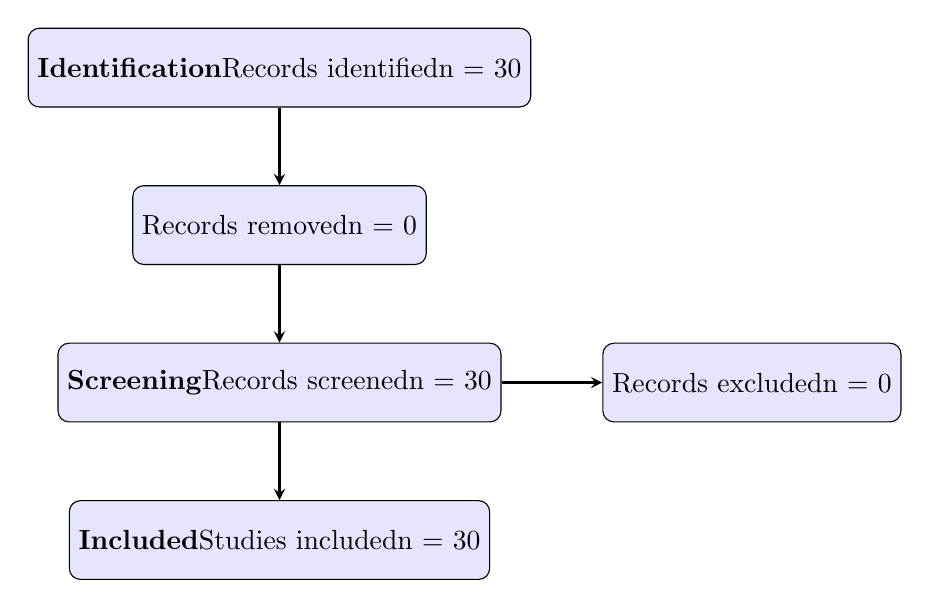
\begin{tikzpicture}[node distance=2cm]

% Identification
\node (identification) [box] {
    \textbf{Identification} \\
    Records identified \\
    n = 30
};

% Records removed
\node (removed) [box, below of=identification] {
    Records removed \\
    n = 0
};

% Screening
\node (screening) [box, below of=removed] {
    \textbf{Screening} \\
    Records screened \\
    n = 30
};

% Records excluded
\node (excluded) [box, right of=screening, xshift=4cm] {
    Records excluded \\
    n = 0
};

% Included
\node (included) [box, below of=screening] {
    \textbf{Included} \\
    Studies included \\
    n = 30
};

% Arrows
\draw [arrow] (identification) -- (removed);
\draw [arrow] (removed) -- (screening);
\draw [arrow] (screening) -- (included);
\draw [arrow] (screening) -- (excluded);

\end{tikzpicture}

\end{document}